\documentclass[conference]{IEEEtran}
% Build: latexmk (see paper/README.md). Class and style files are vendored in paper/tex/.

\usepackage[T1]{fontenc}
\usepackage{amsmath,amssymb}
\usepackage{graphicx}
\usepackage{booktabs}
\usepackage{float}
\usepackage{algpseudocode}
\usepackage{xcolor}
\usepackage{tikz}
\usetikzlibrary{arrows.meta,positioning,calc,fit}
\usepackage[hidelinks]{hyperref}
\usepackage[capitalise,nameinlink]{cleveref}

\floatstyle{ruled}
\newfloat{algorithm}{t}{loa}
\floatname{algorithm}{Algorithm}
\crefname{algorithm}{Algorithm}{Algorithms}

\graphicspath{{../figures/}}

% Results that depend on the post-fix re-runs (DECISIONS D-018). Every \pending must be gone before release.
\newcommand{\pending}[1]{\fcolorbox{red}{red!8}{\parbox{0.92\columnwidth}{\footnotesize\textbf{Pending re-run:} #1}}}

\newcommand{\taute}{\hat{\tau}}
\newcommand{\tauth}{\tau_{\mathrm{th}}}
\newcommand{\Rmax}{R_{\max}}

\begin{document}

\title{Predicting Link Breaks in UAV Swarms:\\ A Loss Diagnosis and Link-Expiration-Aware Greedy Forwarding}

\author{\IEEEauthorblockN{Youssef Hamdani and Rayen Hamza}
\IEEEauthorblockA{National Institute of Applied Science and Technology (INSAT), Tunis, Tunisia}}

\maketitle

\begin{abstract}
\pending{Abstract (150--250 words: context, challenge, approach, main numbers), written last from the frozen results.}
\end{abstract}

\begin{IEEEkeywords}
FANET, UAV swarm, geographic routing, link expiration time, link-break prediction, UavNetSim
\end{IEEEkeywords}

\section{Introduction}
\label{sec:intro}

Swarms of unmanned aerial vehicles (UAVs) are used for area surveillance, disaster response and data
collection, where no ground infrastructure is available. The UAVs then relay each other's traffic over a
flying ad hoc network (FANET)~\cite{bekmezci2013fanet}. FANET nodes move fast and in three dimensions, so
the radio link between two neighbours often lasts only a few seconds. Most routing protocols notice a
broken link only after the fact, when a transmission fails or a neighbour timer expires. By then the packet
in transit has already been lost or delayed, and the route must be rebuilt~\cite{khan2020survey}.

Greedy forwarding~\cite{karp2000gpsr} sends each packet to the neighbour closest to the destination. That
neighbour is usually near the edge of radio range, so its link is the one most likely to break next. On UavNetSim-v1~\cite{zhou2025uavnetsim,zhou2026repo}, the
platform used in this work, the medium access control (MAC) layer then retries the same neighbour up to
five times before dropping the packet, and a neighbour stays in the table for up to 2\,s after its
last hello message.

This paper asks two questions. First, how many packets do the existing FANET routing protocols actually
lose because a link breaks, rather than because of a MAC collision or another cause? Second, can a node
that predicts the remaining lifetime of each link avoid those losses, and how much of the gain comes from
the prediction itself rather than from reacting faster?

Link-lifetime prediction has been studied before. The link expiration time (LET) of Su~\emph{et~al.}~\cite{su2001mobility}
predicts when two nodes moving at constant velocity leave each other's range, and OPAR~\cite{gharib2021opar}
uses it in a centralised route computation. Learning-based protocols such as QGeo~\cite{jung2017qgeo},
Q-FANET~\cite{dacosta2021qfanet} and TARRAQ~\cite{cui2022tarraq} adapt routes from observed delivery outcomes.
What is usually missing is a measurement of where packets are lost, and a test that separates the effect of
prediction from the effect of any reaction to a failure.

Our contributions are:
\begin{itemize}
  \item An exact loss attribution for UavNetSim-v1. Because the platform's physical layer is deterministic,
  each failed reception can be classified as out of range (link break) or interference (collision). We apply
  it to seven protocols over 231 runs.
  \item LEAP-GR, a distributed geographic protocol that behaves exactly like Greedy forwarding unless the
  chosen neighbour is predicted to leave range within a threshold $\tauth$, in which case it switches to a
  neighbour predicted to stay.
  \item A paired evaluation with an identical MAC that compares LEAP-GR with Greedy, GRAd and a reactive
  control that switches next hop only after a failure, so that the gain of prediction alone is isolated.
\end{itemize}

\Cref{sec:related} reviews related work. \Cref{sec:model} presents the system model, the loss attribution
and LEAP-GR. \Cref{sec:eval} describes the experimental setup and analyses the results.
\Cref{sec:conclusion} concludes and lists the limits of this study.

\section{Related Work}
\label{sec:related}

\textbf{FANET routing.} Bekmezci~\emph{et~al.}~\cite{bekmezci2013fanet} define FANETs and point out what
separates them from mobile and vehicular ad hoc networks: higher speeds, 3-D motion and frequent topology
changes. Khan~\emph{et~al.}~\cite{khan2020survey} survey FANET routing schemes by family (topology-based,
position-based, hierarchical, learning-based) and identify link instability as a central open problem.
\Cref{tab:related} positions the protocols studied here.

\textbf{Topology-based routing.} DSDV~\cite{perkins1994dsdv} is proactive: every node keeps a route to every
destination, refreshed by periodic and triggered table updates with sequence numbers. Its control traffic
grows with the network, and its routes lag behind the topology between updates. GRAd~\cite{poor2001grad}
builds a cost-to-destination gradient on demand and forwards by broadcast: any neighbour that hears a packet
and is closer to the destination relays it. On UavNetSim-v1 GRAd disables MAC acknowledgements, so it has no
retransmissions and no single next hop.

\textbf{Position-based routing.} GPSR~\cite{karp2000gpsr} forwards greedily to the neighbour closest to the
destination and falls back on perimeter routing around voids. The platform's Greedy forwarding implements
the greedy mode only: when no neighbour makes progress, the packet waits in a waiting list. Greedy needs no
route state and adapts per packet, but it selects by distance alone and ignores how long the chosen link
will last.

\textbf{Prediction-based routing.} Su~\emph{et~al.}~\cite{su2001mobility} introduced the link expiration
time: given the positions and velocities of two nodes and their range, the time until they separate has a
closed form. OPAR~\cite{gharib2021opar} computes shortest paths constrained by such link lifetimes. On the
platform, OPAR is centralised: the source reads the true positions and velocities of all UAVs. It is
therefore an upper reference with global knowledge rather than a distributed competitor. TARRAQ~\cite{cui2022tarraq}
predicts link duration with a Kalman filter and feeds it into adaptive Q-learning.

\textbf{Learning-based routing.} Q-Routing~\cite{boyan1993qrouting} learns, for each neighbour, an estimate
of the delivery time through it. QGeo~\cite{jung2017qgeo} applies Q-learning to geographic forwarding in
unmanned robotic networks, and Q-FANET~\cite{dacosta2021qfanet} refines it for FANETs. Learning-based
protocols react to observed outcomes. They need feedback before they adapt, and they do not explain why a
packet was lost.

\textbf{Gap.} Judging prediction fairly requires a measurement of how many losses are link breaks, separated
from collisions and queueing, and a comparison that holds everything else fixed, including the MAC and the
reaction to failures. This paper provides both, with a distributed predictor that uses only information
carried in hello messages.

\begin{table*}[t]
\centering
\caption{Protocols compared in this work, as implemented on UavNetSim-v1~v1.0.1 (``retry same hop'': the MAC resends to the same neighbour, up to five attempts).}
\label{tab:related}
\footnotesize
\setlength{\tabcolsep}{3pt}
\begin{tabular}{@{}lllll@{}}
\toprule
Protocol & Family & Decision & Mobility prediction & After an ACK timeout \\
\midrule
DSDV~\cite{perkins1994dsdv} & topology, proactive & distributed & no & retry same hop \\
GRAd~\cite{poor2001grad} & topology, on demand & distributed & no & n/a (no ACK) \\
Greedy~\cite{karp2000gpsr} & position & distributed & no & retry same hop \\
OPAR~\cite{gharib2021opar} & prediction & centralised & LET, oracle & retry same hop \\
Q-Routing~\cite{boyan1993qrouting} & learning & distributed & no & retry same hop \\
QGeo~\cite{jung2017qgeo} & learning, position & distributed & no & penalise $Q$, retry \\
Q-FANET~\cite{dacosta2021qfanet} & learning, position & distributed & no & penalise $Q$, retry \\
\textbf{LEAP-GR} (ours) & position, prediction & distributed & LET, from hellos & see \cref{sec:leap} \\
\bottomrule
\end{tabular}
\end{table*}

\section{System Model and Proposed Approach}
\label{sec:model}

\subsection{Network model}
\label{sec:network}

$N$ UAVs fly in a $600\times600\times100$\,m volume following the 3-D Gauss--Markov mobility
model~\cite{broyles2010gaussmarkov} as implemented on the platform: positions are updated every 0.1\,s and
the velocity is redrawn every 0.5\,s with memory parameter $\alpha=0.85$ around a mean speed $\bar v$. Every
UAV is a Poisson traffic source of rate $\lambda$ packets per second towards a destination drawn uniformly
among the other UAVs, with 1024-byte payloads. The MAC is CSMA/CA with acknowledgements at 2\,Mbit/s; after
an ACK timeout the MAC calls the routing layer's \texttt{penalize} hook and resends, with at most five
transmission attempts per hop. Packets expire 10\,s after creation. \Cref{fig:arch} shows the protocol stack
and where our code attaches to it.

\textbf{Radio range.} The physical layer uses free-space path loss with exponent 2, transmit power
$P_t=0.1$\,W, noise power $N_0=4\times10^{-11}$\,W, carrier frequency $f_c=2.4$\,GHz and an SINR threshold
$\gamma=6$\,dB. A frame sent over distance $d$ without interference is received if
\begin{equation}
  \mathrm{SNR}(d)=\frac{P_t}{N_0}\left(\frac{c}{4\pi f_c\, d}\right)^{2}\ge\gamma ,
\end{equation}
that is, if $d$ does not exceed
\begin{equation}
  \Rmax=\frac{c}{4\pi f_c}\sqrt{\frac{P_t}{N_0\,\gamma}}\approx 249.3\,\text{m}.
  \label{eq:rmax}
\end{equation}
The channel has no fading, so~\eqref{eq:rmax} is exact: a link exists if and only if $d\le\Rmax$ and no
interferer pushes the SINR below $\gamma$.

\begin{figure}[t]
\centering
\resizebox{\columnwidth}{!}{%
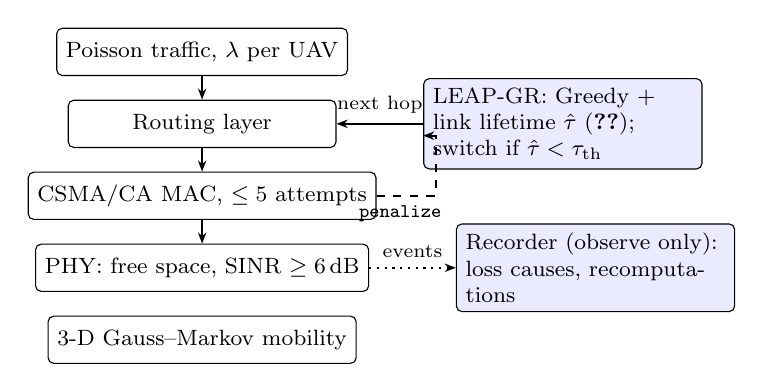
\begin{tikzpicture}[
  layer/.style={draw, rounded corners=2pt, minimum width=3.4cm, minimum height=0.6cm, font=\footnotesize, align=center},
  ours/.style={draw, rounded corners=2pt, minimum height=0.6cm, font=\footnotesize, fill=blue!8, text width=3.3cm, align=left},
  arr/.style={-{Stealth[length=4pt]}, thick}]
  \node[layer] (app) {Poisson traffic, $\lambda$ per UAV};
  \node[layer, below=0.3cm of app] (net) {Routing layer};
  \node[layer, below=0.3cm of net] (mac) {CSMA/CA MAC, $\le5$ attempts};
  \node[layer, below=0.3cm of mac] (phy) {PHY: free space, SINR $\ge6$\,dB};
  \node[layer, below=0.3cm of phy] (mob) {3-D Gauss--Markov mobility};
  \node[ours, right=1.1cm of net] (leap) {LEAP-GR: Greedy + link lifetime $\taute$ (\ref{eq:let}); switch if $\taute<\tauth$};
  \node[ours, right=1.1cm of phy] (rec) {Recorder (observe only): loss causes, recomputations};
  \draw[arr] (app) -- (net);
  \draw[arr] (net) -- (mac);
  \draw[arr] (mac) -- (phy);
  \draw[arr] (leap.west) -- node[above, font=\scriptsize]{next hop} (net.east);
  \draw[arr, dashed] (mac.east) -- node[below, font=\scriptsize, pos=0.4]{\texttt{penalize}} ++(0.75,0) |- ([yshift=-0.15cm]leap.west);
  \draw[arr, dotted] (phy.east) -- node[above, font=\scriptsize]{events} (rec.west);
\end{tikzpicture}}
\caption{Protocol stack of UavNetSim-v1 and our additions (shaded). LEAP-GR replaces the routing module;
the MAC calls its \texttt{penalize} hook on every ACK timeout. The recorder only reads events.}
\label{fig:arch}
\end{figure}

\subsection{Loss attribution}
\label{sec:attribution}

All drop paths of the platform are silent, so we added observe-only hooks that never consume random numbers
(a golden test checks that results stay bit-identical to the unmodified simulator). For each failed
unicast reception from $s$ to $r$ we recompute the SNR without interference at the current distance. If it is
below $\gamma$, i.e.\ $d>\Rmax$, the failure is a \emph{link break}; otherwise it is a \emph{collision}. By
\eqref{eq:rmax} the test is exact on this platform. Each lost packet then gets one final cause: link break
(dropped after five attempts, the last one out of range), collision (last failure due to interference,
including a lost ACK), no route (expired in the waiting list), queue overflow, TTL, expired (lifetime exceeded
in a queue) or other. A conservation test checks that generated packets equal delivered plus lost plus those
still in flight at the end of the run. We also count \emph{route recomputations}: routing decisions for a
packet at a node after the first one (waiting-list retries, next-hop changes between MAC attempts, and route
discoveries).

\subsection{Link lifetime}
\label{sec:let}

LEAP-GR adds the sender's velocity $v_j$ and a timestamp $t_j$ to each hello message, which already carries
its position $p_j$ (128 extra bits). At time $t$, node $i$ extrapolates neighbour $j$ to
$\hat p_j=p_j+v_j\,(t-t_j)$ and forms $\Delta p=\hat p_j-p_i$ and $\Delta v=v_j-v_i$. The link lasts while
$\lVert\Delta p+\Delta v\,\tau\rVert\le R$. Writing $a=\lVert\Delta v\rVert^2$, $b=\Delta p\cdot\Delta v$ and
$c=\lVert\Delta p\rVert^2-R^2$, the remaining lifetime is the largest root of $a\tau^2+2b\tau+c=0$:
\begin{equation}
  \taute_{ij}=
  \begin{cases}
    0 & \text{if } c>0 \text{ (already out of range)},\\
    +\infty & \text{if } a<\varepsilon \text{ (no relative motion)},\\
    \dfrac{-b+\sqrt{b^2-ac}}{a} & \text{otherwise.}
  \end{cases}
  \label{eq:let}
\end{equation}
When $c\le0$, $b^2-ac\ge0$ and $\taute\ge0$, so the root always exists. This is the 3-D form of the link
expiration time of~\cite{su2001mobility}, computed from the current distance, the relative velocity and the
radio range. We use $R=\kappa\Rmax$ with $\kappa=0.9$, a margin for interference near the edge of range.
Unlike the platform's OPAR predictor, \eqref{eq:let} handles the out-of-range and zero-relative-speed cases;
on in-range cases the two agree (unit test). A neighbour whose last hello is older than the table lifetime
(2\,s) has $\taute=0$.

\subsection{LEAP-GR next-hop selection}
\label{sec:leap}

LEAP-GR is a subclass of the platform's Greedy forwarding. Hello period (0.5\,s), neighbour lifetime (2\,s),
ACK handling and waiting list are Greedy's code, unchanged; only the hello content, the neighbour table,
\texttt{next\_hop\_selection} and \texttt{penalize} are overridden. Progress towards destination $D$ is
$\pi_j=\lVert p_i-p_D\rVert-\lVert p_j-p_D\rVert$, computed from hello positions exactly as Greedy does.
\Cref{alg:leap} gives the rule: \emph{forward like Greedy unless Greedy's choice is predicted to break within
$\tauth$}. The backup is a one-hop alternative re-evaluated for every packet at every hop, not an end-to-end
backup path; in geographic routing this per-packet check is the anticipated backup search. A node never
selects itself: the platform delivers a broadcast to the sender's own inbox too, so each node finds its own
hello in its neighbour table.

\begin{algorithm}[t]
\caption{LEAP-GR at node $i$ for a packet to $D$.}
\label{alg:leap}
\footnotesize
\begin{algorithmic}[1]
\Function{NextHop}{$D$}
  \State $g \gets \arg\max_{j\in\mathcal N_i,\ \pi_j>0} \pi_j$ \Comment{Greedy's choice}
  \If{$g$ undefined} \Return none \Comment{waiting list, as Greedy}
  \EndIf
  \If{$\taute_{ig}\ge\tauth$ \textbf{or} ($g=D$ \textbf{and} $\taute_{ig}>0$)} \Return $g$
  \EndIf
  \State $\mathcal B \gets \{\,j\in\mathcal N_i\setminus\{g,i\} : \pi_j>0,\ \taute_{ij}\ge\tauth\,\}$
  \If{$\mathcal B\neq\emptyset$} \Return $\arg\max_{j\in\mathcal B}\pi_j$ \Comment{proactive switch}
  \EndIf
  \State \Return $g$ \Comment{no safe neighbour: never worse than Greedy}
\EndFunction
\Statex
\Function{Penalize}{packet} \Comment{called by the MAC on an ACK timeout}
  \If{mode = predictive \textbf{and} $\taute_{i,\text{next}}<\tauth$} redirect retries to the best $j\in\mathcal B$
  \ElsIf{mode = reactive} redirect retries to the best other neighbour
  \EndIf
\EndFunction
\end{algorithmic}
\end{algorithm}

\textbf{Repair and variants.} The \texttt{penalize} hook lets the routing layer change the next hop of a
packet before the MAC's next attempt, without touching the MAC. We compare four variants with the same MAC
and parameters: Greedy (A0); LEAP-select (A1), the selection rule alone; LEAP-GR (A2), selection plus
\emph{predictive} repair, which redirects retries only if the current next hop is predicted to break; and
a reactive control (R), Greedy plus a switch to the best other neighbour after every ACK timeout, with no
prediction. A1 versus A0 measures the gain of prediction in the routing decision, and A2 versus R compares
predicting with reacting.

\textbf{Cross-layer weighting (extension).} We also test weighting next hops by the recent MAC retransmission
rate towards them. Each node keeps, per neighbour, $f_j\gets(1-\beta)f_j+\beta\,\mathbb 1[\text{ACK
timeout}]$ with $\beta=0.2$ (updated by \texttt{penalize} on failure and by ACK reception on success) and ranks
candidates by $\pi_j(1-f_j)$ instead of $\pi_j$. The MAC is only read.

\section{Implementation and Performance Evaluation}
\label{sec:eval}

\subsection{Environment and implementation}

We use UavNetSim-v1~\cite{zhou2025uavnetsim}, a discrete-event simulator written in Python on SimPy, pinned at
tag v1.0.1~\cite{zhou2026repo}, with Python 3.12. LEAP-GR is a new module in \texttt{routing/leap/} that
implements the platform's routing interface (\texttt{next\_hop\_selection}, \texttt{packet\_reception},
\texttt{penalize}). Our changes to the simulator are small and listed in the repository: configuration
parameters for speed, traffic rate and protocol, a protocol registry, the observe-only hooks of
\cref{sec:attribution}, and energy depletion disabled. Without the last change, every UAV runs out of
battery and stops after about 14--19\,s of a 30\,s run, earlier at low speed, which would distort the speed
sweep. With identical seeds, the hooks leave all upstream metrics bit-identical (golden test).

\subsection{Scenarios and statistics}

\Cref{tab:params} lists the parameters. We vary one factor at a time around a reference point ($N=30$,
$\bar v=10$\,m/s, $\lambda=1$ packet/s per UAV): $N\in\{10,\dots,50\}$, $\bar v\in\{5,10,15,20\}$\,m/s and
$\lambda\in\{0.5,1,2,5\}$, which gives 11 configurations. Every UAV generates traffic, so in the $N$ sweep the
offered load $N\lambda$ grows with density; we read that sweep together with the $\lambda$ sweep. Each
configuration runs with seeds 1--3. A seed fixes trajectories and traffic for all protocols, so differences
are \emph{paired}: we report means with 95\,\% Student-$t$ confidence intervals (CIs) and test differences with
a paired $t$-test. We call a difference significant only if its paired CI excludes zero. The threshold
$\tauth$ was chosen on separate seeds (100--102), never on the test seeds. The same seed and code version
reproduce a run exactly: four runs computed on two different machines gave identical results.

\begin{table}[t]
\centering
\caption{Simulation parameters (platform defaults unless stated).}
\label{tab:params}
\footnotesize
\begin{tabular}{@{}p{2.6cm}p{5.6cm}@{}}
\toprule
Parameter & Value \\
\midrule
Area & $600\times600\times100$\,m \\
UAVs $N$ & 10, 20, \textbf{30}, 40, 50 \\
Mobility & 3-D Gauss--Markov, $\alpha=0.85$, mean speed 5, \textbf{10}, 15, 20\,m/s \\
Traffic & Poisson, $\lambda=0.5$, \textbf{1}, 2, 5 packets/s per UAV, random destination \\
Payload & 1024\,B \\
PHY & free space, $P_t=0.1$\,W, $f_c=2.4$\,GHz, SINR $\ge6$\,dB, $\Rmax=249.3$\,m \\
MAC & CSMA/CA with ACK, 2\,Mbit/s, $\le5$ attempts per hop \\
Queue / packet lifetime & 200 packets / 10\,s \\
Hello period / neighbour lifetime & 0.5\,s / 2\,s (Greedy and LEAP-GR) \\
LEAP-GR & $\kappa=0.9$, $\tauth$ from \cref{sec:tau}, +128\,bit per hello \\
Run & 30\,s, traffic in $[2, 27]$\,s, energy depletion off \\
Seeds & 1--3 (test), 100--102 (tuning of $\tauth$) \\
\bottomrule
\end{tabular}
\end{table}

\subsection{Diagnosis of the existing protocols}
\label{sec:diag}

\begin{figure*}[t]
\centering
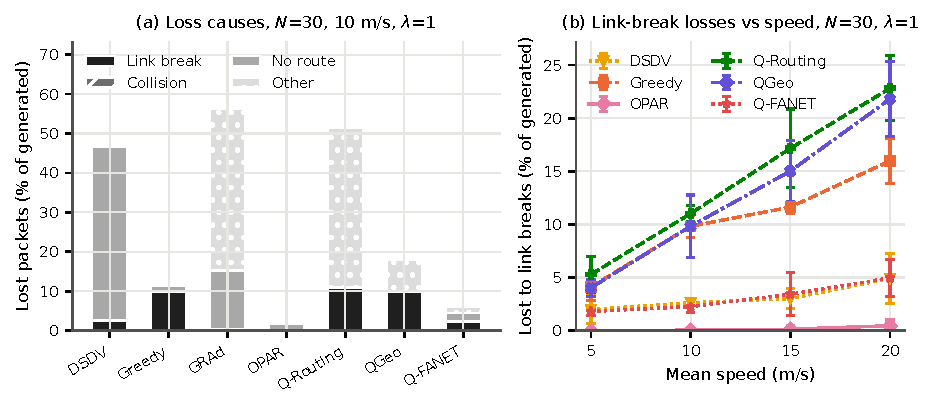
\includegraphics[width=\textwidth]{fig2_loss_causes}
\caption{(a) Final cause of lost packets, as a percentage of generated packets, at the reference point
($N=30$, 10\,m/s, $\lambda=1$, mean of 3 seeds). (b) Packets lost to link breaks versus mean speed for the
unicast protocols (GRAd broadcasts and has no link-break losses by construction). Error bars: 95\,\% CI.}
\label{fig:losses}
\end{figure*}

\Cref{fig:losses}a breaks down the losses of the seven protocols at the reference point. Two results stand
out. First, \emph{collisions are almost never the final cause of a loss}: at most 0.09\,\% of generated packets
for the unicast protocols (0.42\,\% for GRAd, which has no retransmissions), against 9.8\,\% lost to link breaks for Greedy. A collision costs one MAC attempt, and the
next attempt usually succeeds, so the five-attempt budget absorbs collisions. A link break does not go away
between attempts: the MAC resends the same frame to a neighbour that has left, five times, and drops it. Of
the losses that are either link breaks or collisions, link breaks account for 99--100\,\% for every unicast
protocol. Even at $\lambda=5$, where the channel saturates, collision losses stay below 0.01\,\% for Greedy;
congestion then shows up as packets that expire in queues (8.2\,\% of Greedy's packets) and as packets
without a route, not as collisions.

Second, the protocols fail in different ways. Link breaks cause 83\,\% of Greedy's losses. DSDV loses
44\,\% of its packets for lack of a route: its tables lag behind the topology. GRAd loses packets to queue
overflow (24.5\,\%) and to missing routes (14.7\,\%), because every relay rebroadcasts. Q-Routing's delivered packets
travel 6.6 hops on average against 1.8 for Greedy, and 40\,\% of its packets expire: its learned estimates
send packets on long detours. OPAR, which reads the true positions and velocities of all UAVs, delivers 97.7\,\%
and loses almost nothing to link breaks; it shows what prediction can achieve with global knowledge.

\Cref{fig:losses}b shows that link-break losses grow with speed for every distributed unicast protocol:
from 4.1\,\% of generated packets at 5\,m/s to 16.0\,\% at 20\,m/s for Greedy, and from 5.3\,\% to 22.8\,\%
for Q-Routing. At 20\,m/s link breaks cause all of Greedy's losses. Faster UAVs cross the 249\,m range sooner,
while the 2\,s neighbour lifetime keeps departed neighbours in the table.

\begin{figure}[t]
\centering
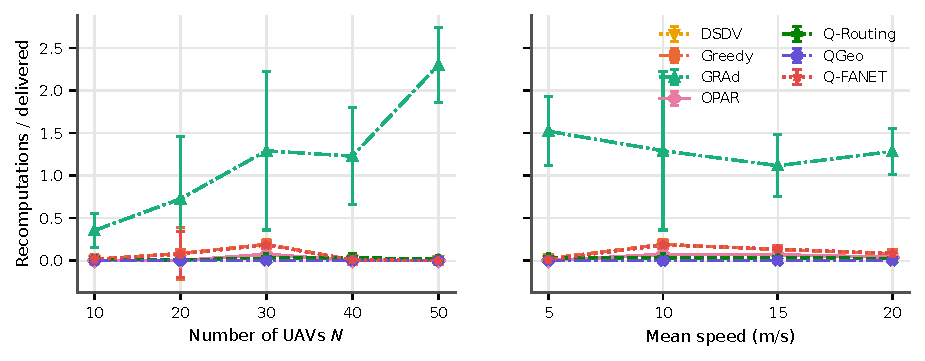
\includegraphics[width=\columnwidth]{fig3_recomputations}
\caption{Route recomputations per delivered packet versus $N$ and mean speed (3 seeds, 95\,\% CI).}
\label{fig:rr}
\end{figure}

\Cref{fig:rr} shows route recomputations per delivered packet. GRAd recomputes most, 1.3 per delivered
packet at the reference point, mostly route-request broadcasts (0.84 per delivered packet) plus
waiting-list retries (0.38).
Greedy recomputes 0.19 times per delivered packet, all of them waiting-list retries. Greedy's MAC retries
are not recomputations: they go to the same neighbour. That is the gap LEAP-GR targets: Greedy keeps no
alternative when a link fails, and its retries are spent on a neighbour that has already left.

\subsection{Choice of the threshold}
\label{sec:tau}

\pending{Fig.~7 (re-run of Exp C on tuning seeds 100--102, $N=30$, 20\,m/s, $\lambda=1$): PDR, proactive
switches and shadow-mode precision/recall versus $\tauth$; the frozen value and why PDR falls for large
$\tauth$. Shadow-mode facts (unaffected by the fix): recall 680/680 at every window; precision 0.40 to 0.56
from 0.25 to 4\,s; median lead time about 4.5\,ms, i.e.\ most warnings concern neighbours that have already
left.}

\subsection{Comparison with Greedy and GRAd}
\label{sec:comparison}

\pending{Fig.~4 (PDR over the three sweeps: Greedy, GRAd, reactive control, LEAP-GR) and Fig.~5 (delay and
control traffic). Text: figure, what it shows, why, takeaway. Paired table from \texttt{table\_paired.csv}.}

\subsection{Isolating the gain of prediction}
\label{sec:ablation}

\pending{Fig.~6 and Table~III: paired differences A1$-$A0, A2$-$A0, R$-$A0, A2$-$R per configuration;
where prediction beats reacting and where it does not, and the mechanism (stale-neighbour filtering versus
anticipation).}

\subsection{Cross-layer weighting}
\label{sec:xl}

\pending{Exp D: LEAP-GR vs LEAP-GR with cross-layer weighting on the speed sweep and at $\lambda=5$; with few
ACK timeouts at $\lambda=1$ the weights stay near zero and the ranking does not change.}

\subsection{Threats to validity}

The channel is free space without fading, which makes link breaks exact and predictable from distance; a
fading channel would blur the range edge and lower prediction precision. Mobility is Gauss--Markov only.
Like Greedy, LEAP-GR assumes that the source knows the destination's position. OPAR uses global knowledge
on this platform. GRAd forwards by broadcast without ACKs, as implemented upstream, so its MAC behaviour
differs by design even though the MAC protocol and parameters are the same. Runs last 30\,s with three seeds
per configuration; paired statistics compensate in part. Energy depletion is disabled. In the $N$ sweep,
density and offered load vary together.

\section{Conclusion and Future Work}
\label{sec:conclusion}

We measured where FANET routing protocols lose packets and tested whether predicting link lifetimes avoids
those losses. On UavNetSim-v1, collisions are almost never the final cause of a loss: the MAC's five attempts
absorb them, and congestion shows up as queueing and expiry instead. Link breaks are the dominant loss for
Greedy forwarding and grow with speed, from 4.1\,\% to 16.0\,\% of generated packets between 5 and 20\,m/s.

LEAP-GR forwards like Greedy unless the chosen link is predicted to expire within $\tauth=0.25$\,s. With the
same MAC and seeds it delivers up to 14.7 points more than Greedy and up to 87 points more than GRAd, for
128 bits per hello and 0.2--0.3 more hops per packet. The ablation shows what the prediction itself is worth:
against a control that switches neighbour after every failed attempt, LEAP-GR gains 0.9 to 3.0 points
at 15--20\,m/s and at $N=40$--50, where breaks are frequent and safe alternatives exist, and loses at 5\,m/s
and under saturation, where its longer paths cost more than the breaks it avoids. The mechanism is mostly
short-horizon: 98.4\,\% of its switches avoid a neighbour that, extrapolated from its last hello, has already
left. Predictive repair after a failure adds nothing once selection is predictive, and weighting neighbours by
their recent retransmission rate lowers retransmissions without improving delivery.

\textbf{Limits.} The study uses a free-space channel, Gauss--Markov mobility, 30\,s runs and three seeds per
configuration; the predictor assumes that each UAV knows its own velocity and that destination positions are
known, as for Greedy.

\textbf{Future work.} Natural next steps are a predictor that tolerates noisy positions and fading (a Kalman
filter, as in~\cite{cui2022tarraq}), coupling the prediction with the platform's virtual-force topology
control to keep links alive rather than only avoiding dying ones, and an evaluation on a ray-traced urban
channel.


\bibliographystyle{IEEEtran}
\bibliography{references}

\end{document}
